\chapter{Introduction to Python}
\label{ch:python}

\begin{center}
\fcolorbox{black}{shadecolor}{%

    \parbox{\textwidth}
    {%
        \small
        {
            This chapter is a basic introduction to programming in Python. If you have previous experience, feel free to proceed to the next chapter.
        }
    }%
}
\end{center}

\section{So, What is Python?}
Python, a programming language globally known for its straightforward syntax, is now one of the most popular languages between developers. And by learning how to master it, you can become one too!

Writing programs is a truly rewarding (and creative) activity. You can have diverse reasons to write a program, varying from solving a difficult data analysis to having genuine fun. Regardless if you like math or not, you do not have to be a great mathematician to be an awesome programmer. 
Even though this chapter is not necessarily intended for professional programmers, advanced programming can be really rewarding (and for the sake of ZX Calculus, it's completely necessary!)

In short you need two main skills to be a programmer:
\begin{itemize}
    \item Know the programming language (Python), including the vocabulary and the grammar. It's like mastering an actual language! You must be able to construct well-formed "sentences".
    \item Tell a story. And by this I mean that you have to combine words and sentences to convey an idea to the reader. In this case, our program is the "story" and the problem we are trying to solve is the "idea".
\end{itemize}

\section{Programming Platform Installation}
First things first. Before getting right into explaining Python's vocabulary, we will explain a simple way to actually start to code in Python. For this, we will use \textbf{Google Colaboratory}. There other ways to download Python but, for the sake of simplicity, we will use an online program. Follow these steps to create a Python file:

\begin{enumerate}
    \item Open Google Chrome and access your Gmail account. If you don't have one, please refer to \href{https://support.google.com/mail/answer/56256?hl=en}{this link} and follow the instructions.
    \item When your account is already set, click on the 9-dot-structure placed on the upper right section of your screen and open Drive. This has a triangle-like logo.
    \item Click on "New" to create a new document. Then, click on "More" and here you will find the option to "Connect more apps".
    \begin{figure}[H]
        \centering
        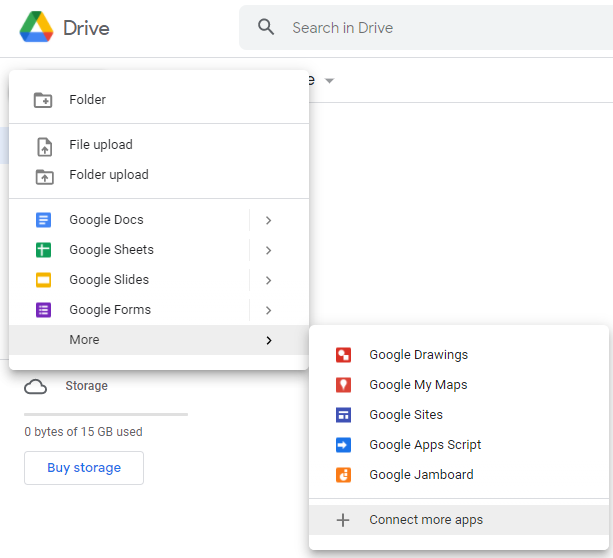
\includegraphics[width = 0.5\textwidth]{Screenshot(15).png}
        \caption{"Connect more apps" option}
        \label{fig:connect-more-apps}
    \end{figure}
    \item A "Google Marketplace Workplace" will appear. Type in the search box "Colaboratory".
    \begin{figure}
        \centering
        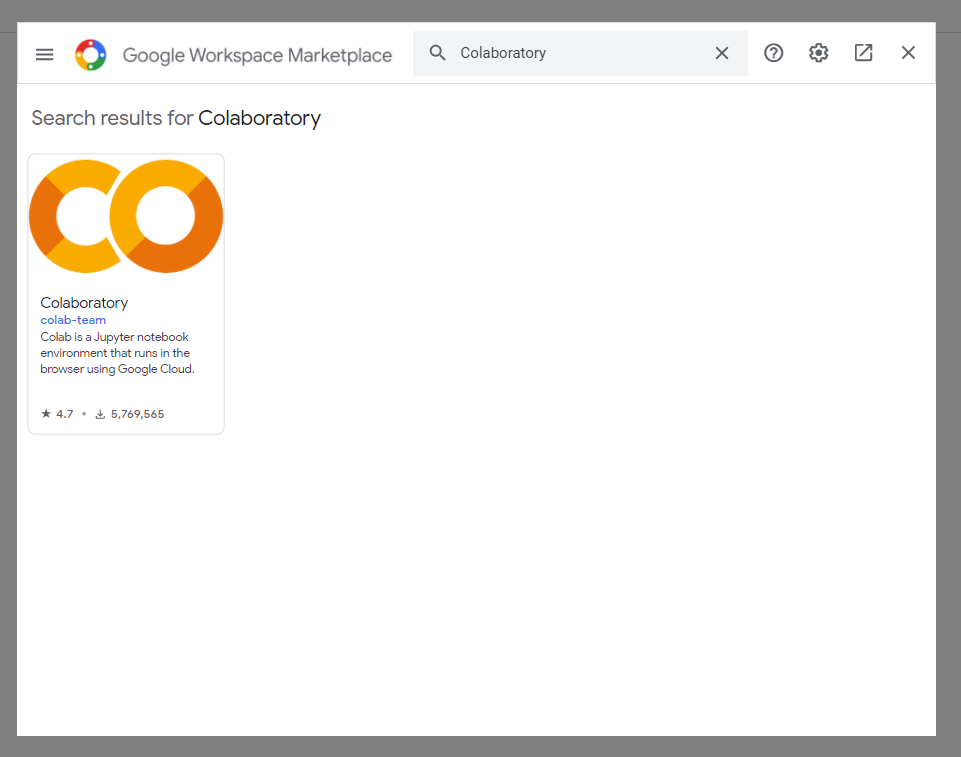
\includegraphics[width=0.5\textwidth]{Figures/Screenshot(18).png}
        \caption{"Google Marketplace Workplace" tab}
        \label{fig:search-colab}
    \end{figure}
    \item Install Google Colaboratory clicking in the blue "Install" button.
    \item To create a new document, press again the "New" button in Drive, then "More" and finally, "Google Colaboratory".
    \begin{figure}[htb]
        \centering
        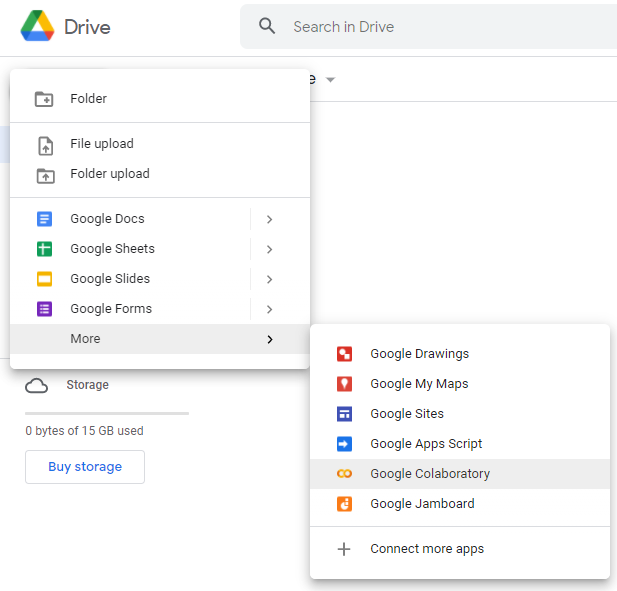
\includegraphics[width=0.5\textwidth]{Figures/Screenshot(21).png}
        \caption{"Google Marketplace Workplace" tab}
        \label{fig:google-marketplace}
    \end{figure}
    \item Congratulations! You have now created a Python file. All the changes you do from now on in the document are automatically saved (yay!).
\end{enumerate}

Now that we have that covered, let's start with the vocabulary and structure of Python programs.

\section{Words and Sentences: Hello, World!}
Imagine that you have a dog. When we want to train a dog, we normally use special words such as "sit", "walk" or "stop". If you talk to the dog and don't use the words you previously taught, they will simply not understand you. For example, if you say, "I wish I could just walk to my best friend's house to play Roblox", what your dog would hear is, "blah blah blah \textit{walk} blah blah blah." 

Similarly, there are words that have a very special meaning to Python. When Python sees these specific words in a program, they have one \textbf{and only one} meaning to Python. Later on, you will also be able to create words with unique meanings on their own called \textit{variables}. In these, you will be able to choose your names for your variables, but this is nothing of the sort with Python's reserved words. 

These reserved words are the following:

\begin{minipage}{\linewidth}
    \begin{spverbatim}
      and, as, assert, break, class, continue, def, del, elif, else, except, finally, for, from, global, if, import, in, is, lambda, nonlocal, not, or, pass, raise, return, try, while, with, yield
    \end{spverbatim}
\end{minipage}

And that's it! The best part is that (unlike a dog) Python is already trained. 

We will learn these reserved words and how they are used in a while, but for now we will focus on the Python equivalent of “speak”. The nice thing about telling Python to speak is that we can even tell it what to say by giving it a message in quotes:

\begin{minted}{python}
print("Hello, World!")
\end{minted}

Our sentence starts with the function print followed by a string of text of our choosing enclosed in single quotes. Try to type it in your Google Colaboratory document! When you have it ready in the cell, click the arrow at the left and you should have the following output:
 \begin{minted}{python}
>>> print("Hello, World!")
Hello, World!
 \end{minted}

You can also print numbers, like this!
\begin{minted}{python}
>>> print(1)
1
\end{minted}

\section{The building blocks of programs}
There are some conceptual patterns that we use to construct programs or, in other words, \textbf{algorithms}. These basic concepts are the following:

\textbf{input} Get data form the user. In our first programs, our input will come from the user typing data on the keyboard.

\textbf{output} Display the results of the program on a screen or store them in a file.

\textbf{sequential execution} Perform statements one after another in the order they are encountered in the program.

\textbf{conditional execution} Check for certain conditions and then execute or skip a sequence of statements.

\textbf{repeated execution} Perform some set of statements repeatedly, usually with some minor variation.

\section{Variables, expressions, and statements}
\subsection{Values and types}
A \textit{value} is a basic component a program works with, such as a letter or a number. The only values we have learned so far are 1 and "Hello, World!"

These values have different \textit{types}: 1 is an integer, and "Hello, World!" is a string (it's called that way because it contains a "string" of letters. These are \textbf{always} enclosed in quotation marks).

If you are not sure what type a value has, you can always receive help from the interpreter:
\begin{minted}{python}
>>> type("Hello, World!")
<class 'str'>

>>> type(43)
<class 'int'>

\end{minted}

There's also another type of value called \texttt{float}, which belongs to numbers with a decimal point.
\begin{minted}{python}
>>> type(5.9)
<class 'float'>
\end{minted}

If numbers are between quotation marks, they are considered strings.
\begin{minted}{python}
>>> type('43')
<class 'str'>
    
>>> type('5.9')
<class 'str'>  
\end{minted}

\subsection{Variables}
One of the most powerful features of a programming language is the ability to manipulate \textit{variables}. A variable is a name that refers to a value. To do this, you just have to assign a value to a variable. A few examples are:
\begin{minted}{python}
>>> greeting = "Hello, my friend!"
>>> age = 16
>>> pi_value = 3.1415926535897931

\end{minted}
This example makes three assignments. The first assigns a string to a new variable named \texttt{greeting}; the second assigns the integer 16 to \texttt{age}; the third assigns the approximate value of pi to $pi_value$.

These values can also be displayed as follows:

\begin{minted}{python}
>>> print(age)
16
    
>>> print(pi_value)
3.1415926535897931
\end{minted}

The type of a variable is the type of the value it refers to.

\begin{minted}{python}
>>> type(greetings)
<class 'str'>
    
>>> type(age)
<class 'int'>
    
>>> type(pi_value)
<class 'float'>
\end{minted}

\subsection{Variable names and keywords}
Variable names can be as long as you want it to be. They can contain both letters and numbers; still, they cannot start with a number. You \textit{can} use uppercase letters to name variables, but it's better to begin with lowercase letters (don't worry, you'll get this later). 
Underscores $(_)$ are often used in multiple-word variables, such as $my_name$.

It is of utmost importance to note that by ANY circumstance, you \textbf{cannot} use a Python keyword as a variable (e.g. class = "Maria's party"). The interpreter uses keywords to recognize the structure of the program, hence they cannot be used as variable names.

Python has 35 keywords:

\begin{minipage}{\linewidth}
    \begin{spverbatim}
        and, as, assert, break, class, continue, def, del, elif, else, except, False, finally, for, from, global, if, import, in, is, lambda, None, nonlocal, not, or, pass, raise, return, True, try, while, with, yield, async, await
    \end{spverbatim}
\end{minipage}

Be sure to take this into account when you create variables!

\subsection{Statements}
A \textit{statement} is defined as a unit of code that the Python interpreter can execute. A program usually contains a sequence of statements. If there is more than one statement, the results appear one at a time as the statements execute. For example:
\begin{minted}{python}
print(1)
x = 2
print(x)
\end{minted}

has the output of:
\begin{minted}{python}
1
2
\end{minted}

\subsection{Operators and Operands}
I know we already said that you don't have to be a great mathematician to be an awesome programmer, but it can definitely help you improve! For this, we have operators. \textit{Operators} are special symbols that represent computations like addition and multiplication. The values the operator is applied to are called \textit{operands}.

The operators \texttt{+}, \texttt{-}, \texttt{*}, \texttt{/}, and \texttt{**} perform addition, subtraction, multiplication, division, and exponentiation respectively. For example:
\begin{minted}{python}
25 + 34
55-35
5*3
10/2
5**2
\end{minted}

The division symbol we see above gives us a \texttt{float} (meaning that the result will be in decimal form). In addition to this, we also have the integer division, in which we will use two slashes \texttt{(//)}.
\begin{minted}{python}
>>> x = 40
>>> x//5
8
\end{minted}

\subsection{Expressions}
An \textit{expression} is a combination of values, variables, and operators. A value all by itself is considered an expression, and so is a variable. Here we have 3 brief examples:
\begin{minted}{python}
    17
    x
    x + 17
\end{minted}

Remember that, in a script, an expression all by itself doesn’t do anything! This is a common
source of confusion for beginners. This can be seen in the example above, as \texttt{17} is not printed. Instead, the result of \texttt{x + 17} can be seen. Try it out in Google Colaboratory!

Another detail we must mention is the \textit{rules of precedence}. You can use acronyms (such as PEMDAS) to remember the rules:
\begin{enumerate}
    \item Parentheses ()
    \item Exponentiation (x**y)
    \item Multiplication and Division (* and / or //)
    \item Addition and Subtraction (+ and -) in order of precedence from left to right
\end{enumerate}

\subsection{String operations}
The \texttt{+} operator works with strings, but it is not addition in the mathematical sense. Instead, it performs \textit{concatenation}, which means joining the strings. For example:
\begin{minted}{python}
>>> a = '100'
>>> b = '200'
>>> print(a+b)
100200
\end{minted}

The \texttt{*} operator also works with strings by multiplying the content of a string by an integer. For example:
\begin{minted}{python}
>>> a = 'Hello '
>>> b = 3
>>> print(a * b)
Hello Hello Hello
\end{minted}

\subsection{Asking the user for input}
If you want to make a "personalized" program by taking the input of the user via the keyboard, there is a way to do so! Python provides a built-in function called \texttt{input} that gets input from the keyboard. When this function is called, the program stops and waits for the user to type something. When the user presses Enter, the program resumes and input returns what the user typed as a string.
\begin{minted}{python}
>>> name = input("What is your name?\n")
Maria
>>> print(name)
Maria
\end{minted}

The sequence at the end of the prompt represents a newline, which is a special character that causes a line break.

\subsection{Comments}
As your program turns out to be more and more complex, you sometimes need to remember some things so you can read it efficiently. Because of this, it is a good idea to add notes into your programs to explain in natural language what a statement/expression is doing. These are \textit{comments}, and in Python we can add them with the hashtag symbol.
\begin{minted}{python}
#find how many seconds are in a specific number of minutes
seconds = minute * 60
\end{minted}

These do not affect your code, so you can write anything you want!

\section{Conditionals}
\subsection{Boolean expressions}
A \textit{boolean expression} is an expression that is either true or false. For this, we use the operator ==, which compares two operands and produces True if they are equal and False otherwise:
\begin{minted}{python}
>>> 5 == 5
True
    
>>> 5 == 10
False
\end{minted}

It is like we are asking to Python, "Are x and y equal?". Remember that one equal symbol (=) is solely for assigning variables.

\texttt{True} and \texttt{False} are special values that belong to the class bool; they are not strings:
\begin{minted}{python}
>>> type(True)
<class 'bool'>

>>> type(False)
<class 'bool'>

\end{minted}

== is only one of all the \textit{comparison operators}. The rest are:
\begin{minted}{python}
    x > y          #x is greater than y
    x < y          #x is less than y
    x >= y         #x is greater than or equal to y
    x <= y         #x is less than or equal to y
    x != y         #x is not equal to y
    x is y         #x is the same as y
    x is not y     #x is not the same as y
\end{minted}

\subsection{Logical operators}
There are three \textit{logical operators}: \texttt{and}, \texttt{or} and \texttt{not}. The meaning of each one is actually straightforward (really similar to their meanings in English). For example:
\begin{minted}{python}
x > 0 and x < 5
\end{minted}
is ONLY true if x is greater than 0 \textit{and} less than 5.

Another example:
\begin{minted}{python}
n%2 == 0 or n%3 == 0
\end{minted}
is true if \textit{either} of the conditions is true (in other words, if n is divisible by 2 \textit{or} 3).

Finally, the \texttt{not} operator negates a boolean expression. Thus:
\begin{minted}{python}
not (x > y)
\end{minted}
is true if x > y is \textit{false} (in other words, if x is less than or equal to y).

\subsection{Conditional execution}
To write useful and effective algorithms, we almost always (if not always) need to include conditions that change how the program is executed according to the circumstances. Because of this is reason is that we use \textit{conditional statements}. The simplest of these is the \texttt{if} statement:
\begin{minted}{python}
if x < 5:
    print("x is lower than 5") #condition
\end{minted}

As you could see in the comment, the boolean expression after the \texttt{if} statement is called a \textit{condition}. For the if statement to have a correct syntax, we must put a colon (:) to end the statement, and the line(s) after the statement must be indented. 

\texttt{if} statements have the same structure as for loops (we will learn about them moreover). Both of these are categorized as \textit{compound statements}, since they are longer than a single code line. 

\section{Alternative execution (if, else)}
We also have the option to specify an \textit{alternative execution}. This means, in English, that "if this statement is \texttt{False}, then we can do this other statement" instead of just passing it off. The syntax would look like the following:
\begin{minted}{python}
if x%3 == 0:
    print("x is divisible by 3")
else:
    print("x is not divisible by 3")
    
\end{minted}
If the remainder when x is divided by 3 is 0, then we know that x is divisible by 3, and the program displays a message to that effect. If the condition is \texttt{False}, the second set of statements is executed.

\subsection{Chained conditionals (if, elif, else)}
Thought only one alternative was not enough? Sometimes, we there are more than two possibilities! \textit{Chained conditionals} allows us to do this.
\begin{minted}{python}
if x < y:
    print("x is less than y")
elif x > y:
    print("x is greater than y")
else:
    print("x and y are equal")
\end{minted}
Fun Fact! \texttt{elif} is an abreviation of "else if". The best part of this is that there are \textbf{no} limit on the number of \texttt{elif} statements we can add. Also, it's not necessary to add an \texttt{else} clause. The only requirement is that it must be at the end but if you don't want it there, o pressure at all!

\begin{center}
\fcolorbox{black}{shadecolor}{%

    \parbox{\textwidth}
    {%
        \small
        {
            \textit{Friendly reminder:}
            Every condition is checked in order. If the first is false, the next is checked, and so on.
        }
    }%
}
\end{center}

\subsection{Nested conditionals}
Level up! One conditional can \textbf{also} be nested within another (surprise!). Thus,
\begin{minted}{python}
if x == y:
    print("x and y are equal")
else:
    if x < y:
        print("x is less than y")
    else:
        print("x is greater than y")
\end{minted}
They are pretty confusing sometimes, so it is recommended to avoid them when you can. 

\section{Functions}
\subsection{Function calls}
A \textit{function} is a named sequence of statements that performs a computation. For example:
\begin{minted}{python}
>>> type(32)
<class 'int'>
\end{minted}
The name of the function is \texttt{type}. The expression in parenthesis is called the \textit{argument} of the function, and the result, for the type function, is the type of argument.

Sometimes, you may hear that the function "takes" an argument and "returns" a result. The result is called the \textit{return value}.

\subsection{Built-in functions}
As it name states, there are some functions that we can use without needing to provide the function definition. These are:
\begin{minted}{python}
>>> max("Hello, World!")
"w"
    
>>> min("Hello, World!")
" "
\end{minted}
The max function tells us the “largest character” in the string (which turns out to be the letter “w”) and the min function shows us the smallest character (which turns out to be a space).

Another very common built-in function is the \texttt{len} function which tells us how many
items are in its argument. If the argument to \texttt{len} is a string, it returns the number of characters in the string.
\begin{minted}{python}
>>> len("Hello, World!")
13
\end{minted}

\subsection{Type conversion functions}
In some specific circumstances, you need to convert values from one type to another. We can do this with built-in functions. 

You can use the \texttt{int} function to convert a float value to an integer.
\begin{minted}{python}
>>> int('32')
32
\end{minted}
When converting an \texttt{int} into a \texttt{float}, it doesn't round it off. Instead, it chops off the fraction part. 
\begin{minted}{python}
>>> int('5.998')
5
\end{minted}
\texttt{float} can convert integers and strings:
\begin{minted}{python}
>>> float(32)
32.0
\end{minted}
Last but not least, \texttt{str} converts its argument to a string:
\begin{minted}{python}
>>> str(32)
'32'
\end{minted}

\subsection{Math functions}
In case someone wants to work with mathematical functions, Python has a \texttt{math} module that provides most of the familiar ones. To use it, we first have to import it:
\begin{minted}{python}
>>> import math
\end{minted}

With this, we created a module object named math. This module object contains the functions and variables defined in the module. To use one of these functions, you must specify the name of the module and the name of the function. Remember to separate these with a dot! 
\begin{minted}{python}
>>> ratio = signal_power / noise_power
>>> decibels = 10 * math.log10(ratio)

>>> radians = 0.7
>>> height = math/sin(radians)
\end{minted}

This first example computes the logarithm base 10 of the signal-to-noise ratio. On the other hand, the second example finds the sine of \texttt{radians}. The conversion of degrees to radians is made first dividing the value by 360 and multiplying it by $2\pi$.
\begin{minted}{python}
>>> degrees = 45
>>> radians = degrees / 360.0 * 2 * math.pi
>>> math.sin(radians)
0.7071067811865476
\end{minted}

In the previous code, the expression \texttt{math.pi} gets the variable \texttt{pi} from the math module.

\subsection{Random numbers}
The \texttt{random} module provides functions that generate pseudorandom numbers (or, in short, "random" numbers).
\begin{minted}{python}
import random

for i in range(10):
    x = random.random()
    print(x)
\end{minted}
This would produce 10 random numbers between 0.0 and up to (but NOT including) 1.0.
\begin{minted}{python}
0.11132867921152356
0.5950949227890241
0.04820265884996877
0.841003109276478
0.997914947094958
0.04842330803368111
0.7416295948208405
0.510535245390327
0.27447040171978143
0.028511805472785867
\end{minted}

\subsection{Adding new functions (def)}
Python also let's your creativity develop! It is also possible to add new functions. A \textit{function definition} defines the name of a brand new function and the sequence of statements that must be executed when the function is called. Here is an example:
\begin{minted}{python}
def printsonglyrics():
    print("I see a little silhouetto of a man")
    print("Scaramouch, Scaramouch, will you do the Fandango!")
\end{minted}
\texttt{def} is a keyword that indicates that this is a function definition. The function, in this case, is \texttt{printsonglyrics}. The empty parenthesis after the name indicate that the function doesn't take any arguments. 

\subsection{Why functions?}
But after all of this explanation, why do we use functions? There are several reasons:
\begin{itemize}
    \item You can name a group of statements, which makes your code shorter and easier to read.
    \item You eliminate repetitive code! The smaller your code is, the better.
    \item Once you write a well-designed function, you can reuse it.
\end{itemize}

\section{Iteration}
\subsection{Updating variables}
A common practice in the world of programming is the use of an assignment statement that updates a variable.
\begin{minted}{python}
x = x + 1
\end{minted}

This means that the final updated value of x will be "the previous value of x added by 1". But before you try to update a variable, you need to initialize it. Like this, for example:
\begin{minted}{python}
>>> x = 0
>>> x = x + 1
\end{minted}

\subsection{The \texttt{while} statement}
Computers are really (really!) good at repeating identical tasks without making errors. To do this, Python provides several features to make this programming process easier. A clear example is the \texttt{while} statement. Here is a simple program to portray what it does:
\begin{minted}{python}
n = 3
while n > 0:
    print(n)
    n = n -1
print("Fire!")
\end{minted}

More formally, the \texttt{while} statement does te following:
\begin{enumerate}
    \item Evaluate the condition (Is it \texttt{True} or \texttt{False}?)
    \item If the condition is false, exit the \texttt{while} statement and continue execution at the next statement.
    \item If the condition is true, execute the body and go back to step 1. 
\end{enumerate}

This makes us introduce a really important concept: a \textit{loop}. Each time we execute the body of the loop is called an \textit{iteration}. Thus, for the above loop, we would say that "It had 3 iterations". 

The body of the loop should change the value of one or more variables so that eventually the condition becomes false and the loop terminates. If this doesn't happen, the loop will repeat forever, resulting in an \textit{infinite loop}.

\subsection{Definite \texttt{for} loops}
Imagine that you have a list. Sometimes, we want to loop through a set of things, and when this is the case, we use a \textit{definite} loop using a \texttt{for} statement. We call the \texttt{while} statement an \textit{indefinite loop} because it simply loops until some condition becomes \texttt{False}. However, the \texttt{for} loop is looping through a known amount of items. Because of this, it runs as many iterations as there are items. Here is an example:
\begin{minted} {python}
friends = ["Rafaela", "Lucia", "Jose"]
for friend in friends:
    print("Happy New Year:", friend)
print("Done!")
\end{minted}

The output would be:
\begin{minted}{python}
Happy New Year: Rafaela
Happy New Year: Lucia
Happy New Year: Jose
Done!
\end{minted}

The \texttt{for} loop is going through the list and executes the body once for each of the three strings of the list.

\section{Strings}
\subsection{What is a string?}
A string is a \textit{sequence} of characters. You can access the characters one at a time with brackets:
\begin{minted}{python}
>>> fruit = "banana"
>>> letter = fruit[1]
\end{minted}

With this, we are extracting the character at index position 1 from the \texttt{fruit} variable and assigns it to the \texttt{letter} variable. The output of the code above is:
\begin{minted}{python}
>>> print(letter)
a
\end{minted}

What? Isn't the first letter of "banana", "b"? In Python, the index is an offset from the beginning of the string, and the offset of the first letter is zero.
\begin{minted}{python}
>>> letter = fruit[0]
>>> print(letter)
b
\end{minted}

"b" is the 0th letter of "banana", while "a" is the 1th letter. 

\subsection{Length of a string (len)}
\texttt{len} is another built-in function that returns the number of characters in a string.
\begin{minted}{python}
>>> fruit = "banana"
>>> len(fruit)
6
\end{minted}

It's really that straightforward! Anoher way you can use this is with negative indices.
\begin{minted}{python}
>>> fruit = "banana"
>>> last = fruit[-1]
>>> print(last)
a
\end{minted}

The expression \texttt{fruit[-1]} denotes the last letter; \texttt{fruit[-2]}, the second to last, and so on.

\subsection{Slicing strings}
As it's name depicts, slicing strings is the act of dividing a string into segments. For example:
\begin{minted}{python}
>>> a = "Maria Fernanda"
>>> print(a[0:5])
Maria
\end{minted}

The operator returns the part of the string from the "n-th" character to the "m-th" character, including the first but excluding the last.

There are also other ways to make the operator even more brief. We can do this using colons. 
\begin{minted}{python}
>>> fruit = "banana"
>>> fruit[:3]
"ban"

>>> fruit[3:]
"ana"
\end{minted}

The colon (:) allude to all the characters before the third one, without including the third one in the first example. The second one uses the same methodology, but with all the last characters from 3 onward. 

\subsection{The \texttt{in} operator}
\texttt{in} is a boolean operator that takes two strings and returns \texttt{True} if the value appears in the string. For example:
\begin{minted}{python}
>>> "a" in "banana"
True

>>> "z" in "banana"
False
\end{minted}

\subsection{String comparison (==)}
To see if two strings are equal, we can use a double equal sign. Like this!
\begin{minted}{python}
if word == "hello"
    print("Hello, my friend!")
\end{minted}

You can also use comparison operators to put strings in alphabetical order:
\begin{minted}{python}
if word < "hello":
    print("Your word, " + word + ", comes before hello.")
elif word > "hello":
    print("Your word, " + word + ", comes after hello.")
else:
    print("Hello, my friend!")
\end{minted}

\section{Lists}
\subsection{What is a list?}
A \textit{list} is a sequence of values. In a string, the values are characters but, in a list, they can be any type. The values in a list are called \textit{elements}. To do a list, you just have to encose the elements in square brackets.
\begin{minted}{python}
[5, 10, 15, 20, 25]
["air", "fire", "water", "earth"]
\end{minted}

The first example is a list of five integers. The second is a list of four strings. You can also \textit{nest} a list within another, like this:
\begin{minted}{python}
["hello", 5.2, 6, [3, 6]]
\end{minted}

Similarly to strings, you can also assign lists a variable:
\begin{minted}{python}
>>> food = ["Hamburger", "Pizza", "Spaghetti"]
>>> ages = ["11, 16, 18, 21]
>>> empty = []
>>> print(food, ages, empty)
["Hamburger", "Pizza", "Gouda"] [11, 16, 18, 21] []
\end{minted}

\subsection{List operations}
The \texttt{+} operator \textit{concatenates} (hope you remember the term!) lists:
\begin{minted}{python}
>>> a = [1, 2, 3]
>>> b = [4, 5, 6]
>>> c = a + b
>>> print(c)
[1, 2, 3, 4, 5, 6]
\end{minted}

The \texttt{*} operator repeats a list depending on the number:
\begin{minted}{python}
>>> [1] * 4
[1, 1, 1, 1]

>>> [4, 5, 6] * 3
[4, 5, 6, 4, 5, 6, 4, 5, 6]
\end{minted}

\section{Dictionaries}
You probably already know pretty well what a dictionary is. And the definition of a \textbf{Python} library is not that far fetched. A \textit{dictionary} is similar to a list, but a little bit more general. In a list, the index positions must be integers, but in a dictionary, indices can be any type (almost).

To give you an example, we will build a dictionary that maps from English to Spanish words, so the keys and the values are \textbf{strings}.

The function \texttt{dict} creates a new dictionary. 
\begin{minted}{python}
>>> dictionary_1 = dict()
>>> print(dictionary_1)
{}
\end{minted}

The curly brackets, \texttt{{}}, says that the dictionary is empty. To add elements to it, you can use square brackets like this:
\begin{minted}{python}
>>> dictionary_1["hello"] = "hola"
\end{minted}
This examples creates an item that maps from the key \texttt{"hello"} to the value \texttt{"uno"}.

\textit{Voila!} If we print the dictionary one more time, we can see a key-value pair with a colon between both:
\begin{minted}{python}
>>> print(dictionary_1)
{"hello" : "hola"}
\end{minted}

You can also add items to a dictionary in an input format. For example, you can create a new dictionary with three items. But if you print it, you might be surprised:
\begin{minted}{python}
>>> dictionary_1 = {"hello": "hola", "goodbye": "adiós", "morning": "mañana"}
>>> print(dictionary_1)
{"hello": "hola", "morning": "mañana", "goodbye": "adiós"}
\end{minted}

The order of the items of a dictionary is unpredictable. Because of this, the key-value pairs will not necessarily be the same. But no worries! It's not a problem at all.Since the elements of a dictionary are never indexed with integer indices, we can use the keys to look up the corresponding values:
\begin{minted}{python}
>>> print(dictionary_1["goodbye"])
"adiós"
\end{minted}

You can also use the \texttt{len} function to know the number of key-value pairs:
\begin{minted}{python}
>>> len(dictionary_1)
3
\end{minted}

\section{Your learning journey}
\textbf{You rock!} You finished the first chapter. We are really proud of you for pushing through! 

Don’t be afraid if the concepts don’t seem to fit together well the first time. We want you to learn Python much more rapidly, but it is like learning a new language that takes time to absorb and understand before it feels natural.By reviewing previous material and even doing some exercises, you will realize that you actually learned a lot of material even if it seems a bit impenetrable at first sight! 

Usually when you are learning your first programming language, there are a few wonderful “Ah hah!” moments where you realize you are making an amazing work.

If something seems particularly hard, there is usually no value in staying up all night and staring at it. \textbf{Take a break}, take a nap, have a snack, watch some Netflix, explain what you are having a problem with to someone (or perhaps your dog), and then come back to it with fresh eyes. I assure you that once you learn the programming concepts in the chapter, you will look back and see that it was all really easy and elegant and it simply took you a bit of time to absorb it.

Using Python is the backbone of quantum computing, so don't be afraid of trying over and over again. In the next chapters, you will immerse into the world of physics and how this strongly related to quantum computing and quantum mechanics. Remember: \textbf{take it slow}. You will get there eventually!

In the next section, you will find some exercises that wrap up everything you made in the chapter. Feel free to complete them to gain confidence about all the knowledge you acquired! If you have any questions about the resolution of one of the problems, do not hesitate to contact us. You can find our email in our website. Good luck and happy coding!

\section{Exercises}
Complete these questions to remember everything you learned in the chapter!

\textbf{Exercise 1.} Define a statement, an expression and a variable.

\textbf{Exercise 2.} Write a program that uses input to ask the user their name and greet them.
\begin{verbatim}
    Enter your name: Maria
    Hello, Maria!
\end{verbatim}

\textbf{Exercise 3.} Write a program that computes the following: If x is greater than z, then print "Congratulations! x is greater than z". If x is smaller than z, print "Try it another time! x is smaller than z". If x and z are equal, print "It's a tie!x and z are equal."

\textbf{Exercise 4.} What is the "def" keyword for in Python?
a) It indicates that the following indented section is to be stored for later use

b) It indicates the start of a new function

c) It is a slang that means "the following code is nice"

d) a and b are correct

e) None of the above

\textbf{Exercise 5.} What will be the output of the following Python program?
\begin{minted}{python}
def myname():
    print("Lucia")
def myfriend():
    print("Fernanda")

myfriend()
myname()
myfriend()
\end{minted}

a) Lucia Fernanda myfriend myname myfriend

b) Lucia Fernanda Lucia

c) Fernanda Lucia myfriend

d) Lucia Lucia Lucia

e) Fernanda Lucia Fernanda

\textbf{Exercise 6.} Write a program that reads numbers repeatedly until the user enters "done".
\begin{minted}{python}
Enter a number: 5
Enter a number: 45
Enter a number: hello
Invalid input. Please write a number.
Enter a number: 6
Enter a number: done
\end{minted}

\textbf{Exercise 7.} Imagine you have this string: s = "dshduyhddsnbobobskj". Find how many times "bob" is repeated using string slicing.

\textbf{Exercise 8.} It is a well known fact that Shakespeare used over 20,000 words in his works all in total. However, how could you determine that in code? Let's use Python for this! List all unique words, sorted in alphabetical order, that are stored in a file \texttt{romeo.txt} containing a subset of Shakespeare's work. To do this efficiently, download a copy of \href{www.py4e.com/code3/romeo.txt}{this file}.

\textbf{Exercise 9.} Why are functions used?

\textbf{Exercise 10.} What is a dictionary? Why are they important in Python?

\section{Further resources}
Do you want to deepen your knowledge in Python? Here we leave you some great sources you can follow. 

\begin{itemize}
    \item \href{https://www.learnpython.org/}{learnpython.org}
    \item \href{https://www.youtube.com/watch?v=Z1Yd7upQsXY&list=PLBZBJbE_rGRWeh5mIBhD-hhDwSEDxogDg}{CS Dojo}
    \item \href{https://www.youtube.com/watch?v=jjqgP9dpD1k&list=PL6beirVtPMMFDD_wzVb2g8CPfVrBuOAkI}{CS50}
    \item 
\end{itemize}